\documentclass{abntex2}
\usepackage[utf8]{inputenc}
\usepackage{graphicx}
\usepackage[num]{abntex2cite}



\titulo{Experimento 5: Amplificador em emissor comum}
\autor{Lucas Rezende de Macedo - 14/0026363\\Jônatas Ribeiro Senna Pires - 14/0090983}
\data{21 de Maio de 2018}
\local{Brasília, Distrito Federal}

\begin{document}

\imprimircapa
\imprimirfolhaderosto

\tableofcontents
\clearpage
\listoffigures
\clearpage

\chapter{Experiências}

 O objetivo do presente experimento consiste na verificação do funcionamento
 de circuitos amplificadores com a utilização de transistores de junção bipolar. Utilizando o circuito da
 figura \ref{fig:circuito1}, foi realizada a experiência 1 e, utilizando o circuito da figura \ref{fig:circuito2},
 foi realizada a experiência 2.

\begin{figure}[h]
  \centering
  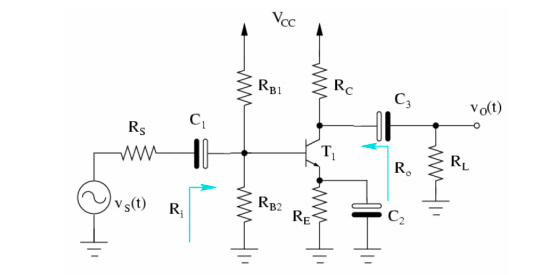
\includegraphics[scale = 0.5]{circuito1.png}
  \caption{Circuito amplificador transistorizado.}
  \label{fig:circuito1}
\end{figure}

\begin{figure}[h]
  \centering
  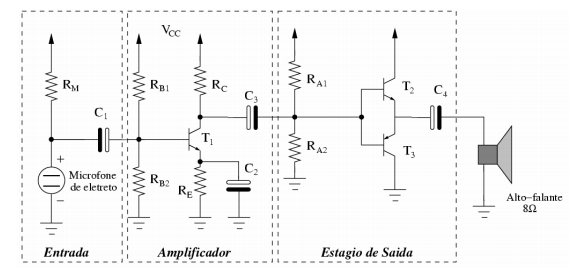
\includegraphics[scale = 0.5]{circuito2.png}
  \caption{Circuito amplificador de sinais de áudio com estágio de saída push-pull.}
  \label{fig:circuito2}
\end{figure}

\section{Experiência}
\subsection{Experiência 1}

Foi montado o circuito da figura \ref{fig:circuito1} com os seguintes parâmetros:
\begin{itemize}
  \item $R_S = 988\Omega $
  \item $R_B_1 = 55,04k\Omega $
  \item $R_B_2 = 36,05k\Omega $
  \item $R_C = 4,6k\Omega$
  \item $R_E = 4,65k\Omega$
  \item $R_L = 46,5k\Omega$
  \item $C_1 = 4,7\mu F$
  \item $C_2 = 47\mu F$
  \item $C_3 = 4,7 \mu F$
  \item $T_1 = BC548$
\end{itemize}

A fonte de tensão foi ajustada para que $V_S$ seja uma onda senoidal de amplitude 20mV e frequência de 1kHz.
\subsubsection{Parte 1}

  Com os valores sugeridos no roteiro do experimento, o transistor não entrou nas zonas de corte ou saturação,
  não sendo necessário o ajuste. Como esperado, a componene AC da saída foi ampliada, assim como demonstra a figura \ref{fig:saida1}.

  \begin{figure}[h]
    \centering
    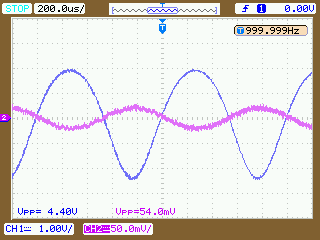
\includegraphics[scale = 0.5]{saida1.png}
    \caption{Formas de onda de entrada (rosa) e saída (azul).}
    \label{fig:saida1}
  \end{figure}

\subsubsection{Parte 2}

  A componente de saída tende a aumentar até chegar à saturação, conforme as figuras \ref{fig:saida2_1}, \ref{fig:saida2_2} e \ref{fig:saida2_3}.

  \begin{figure}[h]
    \centering
    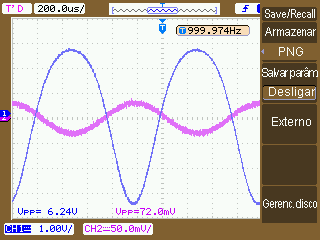
\includegraphics[scale = 0.5]{saida2_1.png}
    \caption{Formas de onda de entrada de 30mV (rosa) e saída (azul).}
    \label{fig:saida2_1}
  \end{figure}
  \begin{figure}[h]
    \centering
    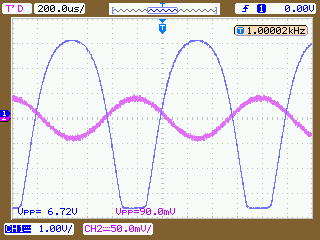
\includegraphics[scale = 0.5]{saida2_2.png}
    \caption{Formas de onda de entrada de 45mV (rosa) e saída (azul).}
    \label{fig:saida2_2}
  \end{figure}
  \begin{figure}[h]
    \centering
    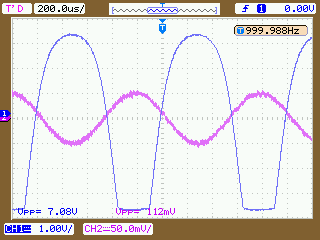
\includegraphics[scale = 0.5]{saida2_3.png}
    \caption{Formas de onda de entrada de 50mV (rosa) e saída (azul).}
    \label{fig:saida2_3}
  \end{figure}

\subsubsection{Parte 3}

  O circuito foi configurado conforme as condicoes da parte 1 e $R_S$ foi ajustado para 0$\Omega$ , e foi notado que houve um aumento no ganho da saída conforme podemos observar na figura \ref{fig:saida_rs}

  \begin{figure}[h]
    \centering
    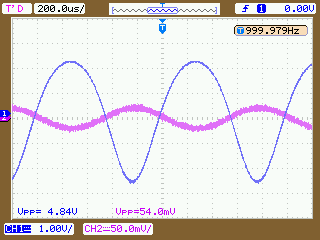
\includegraphics[scale = 0.5]{saida_rs.png}
    \caption{Formas de onda de entrada (rosa) e saída (azul) para $R_S = 0 \Omega$.}
    \label{fig:saida_rs}
  \end{figure}

\subsubsection{Parte 4}
  O circuto foi montado de acordo com as condições da parte 1 e $R_L$ foi ajustado para \infty$\Omega$, e observou-se que a amplitude do sinal de saída diminuiu conforme observado na figura \ref{fig:saida_rl}

  \begin{figure}[h]
    \centering
    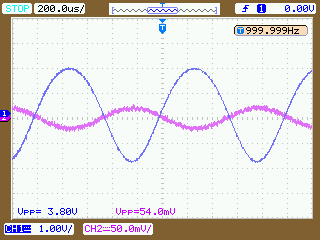
\includegraphics[scale = 0.5]{saida_rl.png}
    \caption{Formas de onda de entrada (rosa) e saída (azul) para $R_L = \infty \Omega$.}
    \label{fig:saida_rl}
  \end{figure}

\subsubsection{Parte 5}

  O circuito foi configurado conforme as condicoes da parte 1, em seguida, a frenquência do sinal de entrada foi variada nos seguintes valores:
  \begin{itemize}
    \item f = 1Hz; Entrada e saída representadas pela figura \ref{fig:freq1}
    \item f = 100Hz; Entrada e saída representadas pela figura \ref{fig:freq2}
    \item f = 2kHz; Entrada e saída representadas pela figura \ref{fig:freq3}
    \item f = 5kHz; Entrada e saída representadas pela figura \ref{fig:freq4}
    \item f = 10kHz; Entrada e saída representadas pela figura \ref{fig:freq5}
    \item f = 20kHz; Entrada e saída representadas pela figura \ref{fig:freq6}
    \item f = 50kHz; Entrada e saída representadas pela figura \ref{fig:freq7}
    \item f = 75kHz; Entrada e saída representadas pela figura \ref{fig:freq8}
    \item f = 100kHz; Entrada e saída representadas pela figura \ref{fig:freq9}
    \item f = 200kHz; Entrada e saída representadas pela figura \ref{fig:freq10}
  \end{itemize}

  \begin{figure}[h]
    \centering
    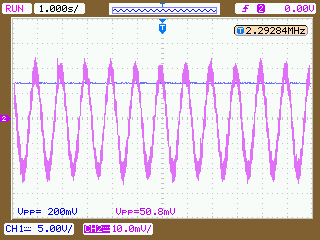
\includegraphics[scale = 0.5]{freq_1.png}
    \caption{Formas de onda de entrada (rosa) e saída (azul) para a frequência de 1Hz.}
    \label{fig:freq1}
  \end{figure}

  \begin{figure}[h]
    \centering
    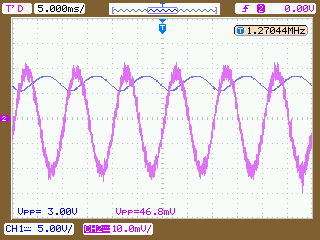
\includegraphics[scale = 0.5]{freq_100.png}
    \caption{Formas de onda de entrada (rosa) e saída (azul) para a frequência de 100Hz.}
    \label{fig:freq2}
  \end{figure}

  \begin{figure}[h]
    \centering
    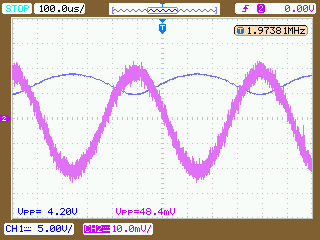
\includegraphics[scale = 0.5]{freq_2k.png}
    \caption{Formas de onda de entrada (rosa) e saída (azul) para a frequência de 2kHz.}
    \label{fig:freq3}
  \end{figure}

  \begin{figure}[h]
    \centering
    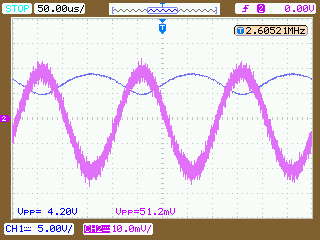
\includegraphics[scale = 0.5]{freq_5k.png}
    \caption{Formas de onda de entrada (rosa) e saída (azul) para a frequência de 5kHz.}
    \label{fig:freq4}
  \end{figure}

  \begin{figure}[h]
    \centering
    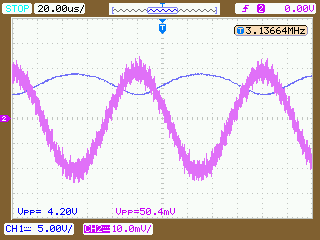
\includegraphics[scale = 0.5]{freq_10k.png}
    \caption{Formas de onda de entrada (rosa) e saída (azul) para a frequência de 10kHz.}
    \label{fig:freq5}
  \end{figure}

  \begin{figure}[h]
    \centering
    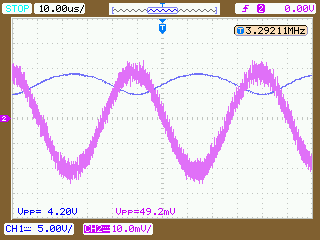
\includegraphics[scale = 0.5]{freq_20k.png}
    \caption{Formas de onda de entrada (rosa) e saída (azul) para a frequência de 20kHz.}
    \label{fig:freq6}
  \end{figure}

  \begin{figure}[h]
    \centering
    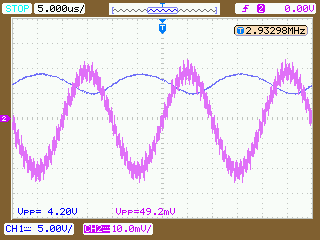
\includegraphics[scale = 0.5]{freq_50k.png}
    \caption{Formas de onda de entrada (rosa) e saída (azul) para a frequência de 50kHz.}
    \label{fig:freq7}
  \end{figure}

  \begin{figure}[h]
    \centering
    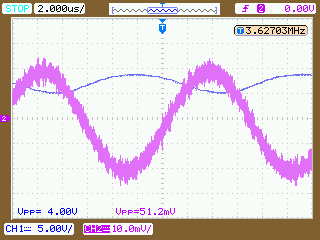
\includegraphics[scale = 0.5]{freq_75k.png}
    \caption{Formas de onda de entrada (rosa) e saída (azul) para a frequência de 75kHz.}
    \label{fig:freq8}
  \end{figure}

  \begin{figure}[h]
    \centering
    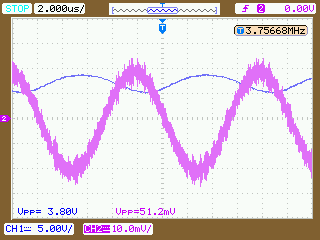
\includegraphics[scale = 0.5]{freq_100k.png}
    \caption{Formas de onda de entrada (rosa) e saída (azul) para a frequência de 100kHz.}
    \label{fig:freq9}
  \end{figure}

  \begin{figure}[h]
    \centering
    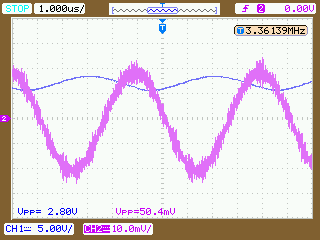
\includegraphics[scale = 0.5]{freq_200k.png}
    \caption{Formas de onda de entrada (rosa) e saída (azul) para a frequência de 200kHz.}
    \label{fig:freq10}
  \end{figure}

  \clearpage

\subsection{Experiência 2}

Foi montado o circuito da figura \ref{fig:circuito2} com os seguintes parâmetros:
\begin{itemize}
  \item $R_S = 988\Omega $
  \item $R_B_1 = 55,04k\Omega $
  \item $R_B_2 = 36,05k\Omega $
  \item $R_C = 4,6k\Omega$
  \item $R_E = 4,65k\Omega$
  \item $R_M = 988\Omega$
  \item $R_{A1} = 100k\Omega$
  \item $R_{A2} = 100k\Omega$
  \item $C_1 = 4,7 \mu F$
  \item $C_2 = 47 \mu F$
  \item $C_3 = 4,7 \mu F$
  \item $C_4 = 220 \mu F$
  \item $T_1 = BC548$
  \item $T_2 = TIP31$
  \item $T_3 = TIP32$
\end{itemize}

O amplificador de som foi testado com gentis toques, sopros e falando, e colocando música no microfone.

\chapter{Discussão}

\section{Questão 1 - Análise do circuito 1}


\section{Questão 2 - Análise da saída do amplificador de áudio}

O amplificador apresentou demasiada distorção do som e ruído para os metodos de teste utilizados, principalmente a música que teve sua melodia profundamente prejudicda. A baixa qualidade do som pode ter sido causada por irregularidades na membrana do microfone da caixa de som, por variações nos valores dos capacitores, pelo sinal de entrada passar do ponto de operação do amplificador ou porque o $\lambda$ dos transistores não é igual a 0.

\clearpage

\section*{Referências}

[1] SEDRA, Adel S.; SMITH, Kenneth Carless. Microelectronic circuits. New York: Oxford University Press, 1998.

[2] RAZAVI, Behzad; BEHZAD, Razavi. RF microelectronics. New Jersey: Prentice Hall, 1998.

\end{document}
